%\documentclass[10pt,times,twocolumn]{paper}
\documentclass[english,aps,prd,nofootinbib]{revtex4-1}
%\documentclass[twocolumn,english,aps,prd,nofootinbib]{revtex4-1}
\usepackage{CJK}

%\usepackage{tikz}
\usepackage{amsfonts}
\usepackage{amsmath}
\usepackage{hyperref}
%\usepackage{hyperref}
\usepackage{amssymb}
\usepackage{xcolor}
\usepackage{relsize}%\mathlarger command 
%\usetikzlibrary{arrows,decorations.markings}
\usepackage[bottom]{footmisc}

%\usepackage{newtxtext}
%\usepackage{multicol}
%\usepackage{comment}
\usepackage{tikz}
\usetikzlibrary{calc,arrows,decorations.markings}

%\usetikzlibrary{tikzmark,fit}

\usepackage{units}

%%%%%%%%%%%%%%%%%%%%%%%%%%%%%%%%%%%%%%%%%%%%%%%%%%%%%%%%%%

\newcommand{\jha}[1]{\textbf{\textcolor{red}{(#1 --jha)}}}
\newcommand{\inti}[1]{\textbf{\textcolor{green}{(#1 --El Jefe)}}}
\newcommand{\be}{\begin{equation}}
\newcommand{\ee}{\end{equation}}
\newcommand{\bea}{\begin{equation} \begin{aligned}}
\newcommand{\eea}{\end{aligned} \end{equation} }
\newcommand{\bi}{\begin{itemize}}
\newcommand{\ei}{\end{itemize}}

\renewcommand{\textfraction}{0.10}
\renewcommand{\topfraction}{0.90}
\renewcommand{\bottomfraction}{0.90}
\renewcommand{\floatpagefraction}{0.65}

\usepackage{xspace}

\newcommand{\la}{\lambda}
\renewcommand{\b}{\beta}

\newcommand{\al}{\alpha}
\newcommand{\eps}{\epsilon}
\newcommand{\D}{\Delta}
\renewcommand{\l}{\lambda}
\renewcommand{\th}{\theta}
\newcommand{\lp}{\left(}
\newcommand{\rp}{\right)}
\newcommand{\Dp}{\mathcal{D}\phi}
\newcommand{\del}{\partial}
\newcommand{\grad}{\vec{\nabla}}
\newcommand{\Div}{\vec{\nabla} \cdot }
\newcommand{\curl}{\vec{\nabla} \times }
\newcommand{\Tr}{\text{Tr} \ }
\newcommand{\lag}{\mathcal{L}}
\newcommand{\delb}{\bar{\del}}



%%%%%%%%%%%%%%%%%%%%%%%%%%%%%%%%%%%%%%%%%%%%%%%%%%%%%%%%%%

\usepackage{color}
\usepackage{graphicx}
\usepackage[space]{grffile}
%\usepackage{indentfirst}
\usepackage{verbatim}
\usepackage{amsmath}
\usepackage{amssymb}
\usepackage{wasysym}
\usepackage[caption=false]{subfig}
\usepackage{url}
\usepackage{bbold}
\usepackage{slashed}
\usepackage{epstopdf}
\usepackage{braket}
\usepackage{float}

%\usepackage{biblatex}

\newcommand{\aaps}{{Astron.~Astrophys.~Supp.}}
\newcommand{\physrep}{{Physics~Reports}}
\newcommand{\araa}{{Annu.~Rev.~Astron.~Astrophys.}}
\newcommand{\aap}{{Astron.~Astrophys.}}
\newcommand{\apjl}{{Astrophys.~J.~Lett.}}
\newcommand{\apjs}{{Astrophys.~J.~Supp.}}
\newcommand{\aj}{{Astron.~J.}}
%\newcommand{\apj}{The Astrophysics Journal}
\newcommand{\mnras}{{Mon.~Not.~R.~Astron.~Soc.}}
\newcommand{\aapr}{{Astronomy and Astrophysics Reviews}}

\DeclareRobustCommand{\Sec}[1]{Sec.~\ref{#1}}
\DeclareRobustCommand{\Secs}[2]{Secs.~\ref{#1} and \ref{#2}}
\DeclareRobustCommand{\App}[1]{App.~\ref{#1}}
\DeclareRobustCommand{\Tab}[1]{Table~\ref{#1}}
\DeclareRobustCommand{\Tabs}[2]{Tables~\ref{#1} and \ref{#2}}
\DeclareRobustCommand{\Fig}[1]{Fig.~\ref{#1}}
\DeclareRobustCommand{\Figs}[2]{Figs.~\ref{#1} and \ref{#2}}
\DeclareRobustCommand{\Eq}[1]{Eq.~(\ref{#1})}
\DeclareRobustCommand{\Eqs}[2]{Eqs.~(\ref{#1}) and (\ref{#2})}
\DeclareRobustCommand{\Ref}[1]{Ref.~\cite{#1}}
\DeclareRobustCommand{\Refs}[1]{Refs.~\cite{#1}}
\DeclareMathAlphabet\mathbfcal{OMS}{cmsy}{b}{n}

\newcommand{\boundellipse}[3]% center, xdim, ydim
{[black,fill=blue!30] (#1) ellipse (#2 and #3)
}
\newcommand{\boundellipseW}[3]% center, xdim, ydim
{[white,fill=white] (#1) ellipse (#2 and #3)
}
\newcommand*{\Scale}[2][4]{\scalebox{#1}{$#2$}}%
\newcommand*{\Resize}[2]{\resizebox{#1}{!}{$#2$}}%
\DeclareMathOperator*{\Motimes}{\text{\raisebox{0.25ex}{\scalebox{0.8}{$\bigotimes$}}}}
%\usepackage{mathabx,graphicx}
\def\Circlearrowleft{\ensuremath{%
  \rotatebox[origin=c]{180}{$\circlearrowleft$}}}
\def\Circlearrowright{\ensuremath{%
  \rotatebox[origin=c]{180}{$\circlearrowright$}}}
\def\CircleArrowleft{\ensuremath{%
  \reflectbox{\rotatebox[origin=c]{180}{$\circlearrowleft$}}}}
\def\CircleArrowright{\ensuremath{%
  \reflectbox{\rotatebox[origin=c]{180}{$\circlearrowright$}}}}



\begin{document}

\thispagestyle{empty}

\begin{figure}
\centering
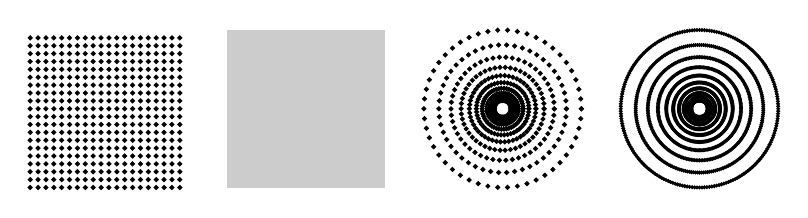
\begin{tikzpicture}
    [%%%%%%%%%%%%%%%%%%%%%%%%%%%%%%
        dot/.style={circle,draw=black, fill,inner sep=0.5pt},
    ]%%%%%%%%%%%%%%%%%%%%%%%%%%%%%%

%\node[circle,draw=white, fill,inner sep=2.5pt] at (0,0.001){};

\foreach \x in {0,0.1,...,2.0}{
	\foreach \y in {0,0.1,...,2.0}{
		\node[dot] at (\x,\y){ };
	}
}

\fill[black!20!white] (3.0-0.5,0.0) rectangle (5.0-0.5,2.0);

\foreach \r in {18,21,...,45}{
	\foreach \y in {0,.2,...,10.0}{
		\node[dot] at ($(
		{6+tan(\r)^2*cos(\y*36.)},
		{1+tan(\r)^2*sin(\y*36.)}
		)$){ };
%		\node[circle,draw=blue, fill,inner sep=2.5pt] at (\x,0){ };
%	    \draw[thick] (\x,\y) -- (\x+1,\y);
%	    \draw[thick] (\x,\y) -- (\x,\y+1);
%		\node[circle,inner sep=0.75pt,draw] at (\x+.5,\y){ };
%		\node[circle,inner sep=0.75pt,draw] at (\x,\y+.5){ };
	}
}

\foreach \r in {18,21,...,45}{
	\foreach \y in {0,.05,...,10.0}{
		\node[circle,draw=black, fill,inner sep=0.01mm] at ($
		(
		{9-0.5+tan(\r)^2*cos(\y*36.)},
		{1+0.0+tan(\r)^2*sin(\y*36.)}
		)$){ };
%		\node[circle,draw=blue, fill,inner sep=2.5pt] at (\x,0){ };
%	    \draw[thick] (\x,\y) -- (\x+1,\y);
%	    \draw[thick] (\x,\y) -- (\x,\y+1);
%		\node[circle,inner sep=0.75pt,draw] at (\x+.5,\y){ };
%		\node[circle,inner sep=0.75pt,draw] at (\x,\y+.5){ };
	}
}


\end{tikzpicture}
\end{figure}

\begin{comment}
\begin{figure}
\centering
\begin{tikzpicture}
    [%%%%%%%%%%%%%%%%%%%%%%%%%%%%%%
        dot/.style={circle,draw=black, fill,inner sep=0.5pt},
    ]%%%%%%%%%%%%%%%%%%%%%%%%%%%%%%

%\node[circle,draw=white, fill,inner sep=2.5pt] at (0,0.001){};

\foreach \x in {0,0.1,...,2.0}{
	\foreach \y in {0,0.1,...,2.0}{
		\node[dot] at (\x,\y){ };
	}
}

\fill[black!40!white] (3.0-0.5,0.0) rectangle (5.0-0.5,2.0);

\foreach \r in {0.05,0.15,...,1.0}{
	\foreach \y in {0,.2,...,10.0}{
		\node[dot] at ($({+1+\r*cos(\y*36.)},{-2+0.5+\r*sin(\y*36.)})$){ };
%		\node[circle,draw=blue, fill,inner sep=2.5pt] at (\x,0){ };
%	    \draw[thick] (\x,\y) -- (\x+1,\y);
%	    \draw[thick] (\x,\y) -- (\x,\y+1);
%		\node[circle,inner sep=0.75pt,draw] at (\x+.5,\y){ };
%		\node[circle,inner sep=0.75pt,draw] at (\x,\y+.5){ };
	}
}

\foreach \r in {1,2.5,...,23}{
	\foreach \y in {0,.05,...,10.0}{
		\node[circle,draw=black, fill,inner sep=0.01mm] at ($
		({4-0.5+tan(\r)**2*cos(\y*36.)},{-2+0.5+tan(\r)**2*sin(\y*36.)})$){ };
%		\node[circle,draw=blue, fill,inner sep=2.5pt] at (\x,0){ };
%	    \draw[thick] (\x,\y) -- (\x+1,\y);
%	    \draw[thick] (\x,\y) -- (\x,\y+1);
%		\node[circle,inner sep=0.75pt,draw] at (\x+.5,\y){ };
%		\node[circle,inner sep=0.75pt,draw] at (\x,\y+.5){ };
	}
}


\end{tikzpicture}
\end{figure}
\end{comment}


\end{document}